\author{Fabrizio}
The STM32D407VG-Discovery board is equipped with a MP45DT02 MEMS microphone and a CS43L22 DAC for audio acquisition and processing. In this project, we will use these devices to detect the sounds' frequency, which will determine the commands given to the robot.

\subsection{The MP45DT02 microphone}
The MP45DT02-M is a compact, low-power, topport, omnidirectional, digital MEMS microphone. It's soldered on the top of the STM32F407G-DISC1 board, in the bottom-right corner.
\begin{figure}[H]
	\centering
	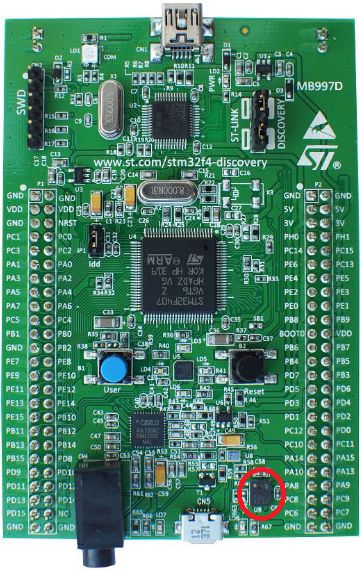
\includegraphics
	{files/images/board_view}
	\caption{View of the upper surface of the board, with the microphone highlighted in the circle.}
\end{figure}

In its bottom surface, it has 6 pins:
\begin{enumerate}
	\item \textbf{GND} - Connected to the GND of the board
	\item \textbf{LR} - Channel selection: used because the microphone is designed to allow stereo audio capture. If it is connected to GND, the MP45DT02 is placed in "left" channel mode: a sample is latched to the data output pin (PDM) on a falling edge of the clock, while on the rising clock edge, the output is set to high impedance. If the LR pin is connected to Vdd then the device operates in "right" channel mode and the MP45DT02 latches it's sample to PDM on a clock rising edge, setting the pin to high impedance on the falling edge of the clock.
	\item \textbf{GND} - Connected to the GND of the board
	\item \textbf{CLK} - Synchronization input clock: this pin is connected to the PB10 port of the board. The clock signal determines the sampling frequency.
	\item \textbf{DOUT} - PDM Data Output. Connected to the PC03 pin of the board's GPIO.
	\item \textbf{VDD} - Power supply.
\end{enumerate}

\begin{figure}[H]
	\centering
	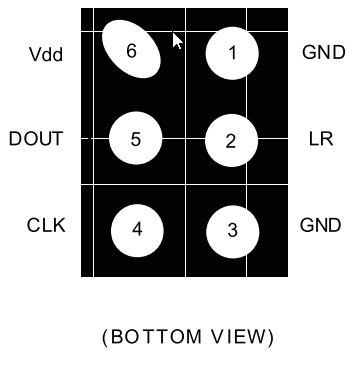
\includegraphics
	{files/images/mic_bottom_pins}
	\caption{Pins on the bottom of the microphone.}
\end{figure}
